%%%%%%%%%%%%%%%%%%%%%%%%%%%%%%%%%%%%%%%%%
% Masters/Doctoral Thesis 
% LaTeX Template
% Version 2.4 (22/11/16)
%
% This template has been downloaded from:
% http://www.LaTeXTemplates.com
%
% Version 2.x major modifications by:
% Vel (vel@latextemplates.com)
%
% This template is based on a template by:
% Steve Gunn (http://users.ecs.soton.ac.uk/srg/softwaretools/document/templates/)
% Sunil Patel (http://www.sunilpatel.co.uk/thesis-template/)
%
% Template license:
% CC BY-NC-SA 3.0 (http://creativecommons.org/licenses/by-nc-sa/3.0/)
%
%%%%%%%%%%%%%%%%%%%%%%%%%%%%%%%%%%%%%%%%%

%----------------------------------------------------------------------------------------
%	PACKAGES AND OTHER DOCUMENT CONFIGURATIONS
%----------------------------------------------------------------------------------------

\documentclass[
11pt, % The default document font size, options: 10pt, 11pt, 12pt
oneside, % Two side (alternating margins) for binding by default, uncomment to switch to one side
%catalan,
english,
%spanish,
singlespacing, % Single line spacing, alternatives: onehalfspacing or doublespacing
%draft, % Uncomment to enable draft mode (no pictures, no links, overfull hboxes indicated)
%nolistspacing, % If the document is onehalfspacing or doublespacing, uncomment this to set spacing in lists to single
%liststotoc, % Uncomment to add the list of figures/tables/etc to the table of contents
%toctotoc, % Uncomment to add the main table of contents to the table of contents
%parskip, % Uncomment to add space between paragraphs
%nohyperref, % Uncomment to not load the hyperref package
headsepline, % Uncomment to get a line under the header
%chapterinoneline, % Uncomment to place the chapter title next to the number on one line
%consistentlayout, % Uncomment to change the layout of the declaration, abstract and acknowledgements pages to match the default layout
]{MastersDoctoralThesis} % The class file specifying the document structure

\usepackage[utf8]{inputenc} % Required for inputting international characters
\usepackage[T1]{fontenc} % Output font encoding for international characters
\usepackage{eurosym}
\usepackage{footnote}
\usepackage{palatino} % Use the Palatino font by default
\usepackage{babel}
\usepackage[backend=bibtex,style=numeric,natbib=true,sorting=none]{biblatex}
\usepackage{multirow}
\usepackage{float}
\usepackage{tabularx}
\usepackage{listings}
\usepackage{xcolor}
\usepackage{appendix}
\usepackage{datetime}
\usepackage{array}
\usepackage{mathtools}
%\usepackage{fontspec}
%\setmainfont{Helvetica Neue Light}

\addbibresource{main.bib} % The filename of the bibliography

\usepackage[autostyle=true]{csquotes} % Required to generate language-dependent quotes in the bibliography

\newdate{date}{02}{03}{2018}
\date{\displaydate{date}}

%----------------------------------------------------------------------------------------
%	MARGIN SETTINGS
%----------------------------------------------------------------------------------------

\geometry{
	paper=a4paper, % Change to letterpaper for US letter
	inner=2.5cm, % Inner margin
	outer=3cm, % Outer margin
	bindingoffset=.5cm, % Binding offset
	top=1.5cm, % Top margin
	bottom=1.5cm, % Bottom margin
	%showframe, % Uncomment to show how the type block is set on the page
}

%----------------------------------------------------------------------------------------
%	THESIS INFORMATION
%----------------------------------------------------------------------------------------

\thesistitle{Skyscanner offer and demand comparison} % Your thesis title, this is used in the title and abstract, print it elsewhere with \ttitle
\supervisor{Javier Arias} % Your supervisor's name, this is used in the title page, print it elsewhere with \supname
\examiner{} % Your examiner's name, this is not currently used anywhere in the template, print it elsewhere with \examname
\degree{Computer Engineering Degree} % Your degree name, this is used in the title page and abstract, print it elsewhere with \degreename
\author{Fèlix Arribas} % Your name, this is used in the title page and abstract, print it elsewhere with \authorname
\addresses{} % Your address, this is not currently used anywhere in the template, print it elsewhere with \addressname

\def \universitysupervisor{Maria José Casañ}

\keywords{} % Keywords for your thesis, this is not currently used anywhere in the template, print it elsewhere with \keywordnames
\university{Universitat Politècnica de Catalunya (UPC)} % Your university's name and URL, this is used in the title page and abstract, print it elsewhere with \univname
\department{\href{https://www.essi.upc.edu/}{Software Engineering and Information Systems department}} % Your department's name and URL, this is used in the title page and abstract, print it elsewhere with \deptname
\group{\href{https://www.essi.upc.edu/}{ESSI}} % Your research group's name and URL, this is used in the title page, print it elsewhere with \groupname
\faculty{\href{http://www.fib.upc.edu}{Facultat d'Informàtica de Barcelona (FIB)}} % Your faculty's name and URL, this is used in the title page and abstract, print it elsewhere with \facname

\def \company{Skyscanner}
\def \tribe{Marketplace Engine tribe}
\def \squad{DeLorean squad}

\AtBeginDocument{
\hypersetup{pdftitle=\ttitle} % Set the PDF's title to your title
\hypersetup{pdfauthor=\authorname} % Set the PDF's author to your name
\hypersetup{pdfkeywords=\keywordnames} % Set the PDF's keywords to your keywords
\hypersetup{linkcolor=black}
}

\newcolumntype{L}{>{\centering}m{0.75cm}}
\newcolumntype{M}{m{9cm}}
\newcolumntype{T}{m{12cm}}

\newcommand\tab[1][0.75cm]{\hspace*{#1}}


\colorlet{punct}{red!60!black}
\definecolor{background}{HTML}{EEEEEE}
\definecolor{delim}{RGB}{20,105,176}
\colorlet{numb}{magenta!60!black}

\lstdefinelanguage{json}{
    basicstyle=\normalfont\ttfamily,
    numbers=left,
    numberstyle=\scriptsize,
    stepnumber=1,
    numbersep=8pt,
    showstringspaces=false,
    breaklines=true,
    frame=lines,
    backgroundcolor=\color{background}
}

\lstdefinelanguage{java}{
    basicstyle=\normalfont\ttfamily,
    numbers=left,
    numberstyle=\scriptsize,
    stepnumber=1,
    numbersep=8pt,
    showstringspaces=false,
    breaklines=true,
    frame=lines,
    backgroundcolor=\color{background}
}

\setlength{\parindent}{0pt}

\begin{document}
\selectlanguage{english}

\frontmatter % Use roman page numbering style (i, ii, iii, iv...) for the pre-content pages

\pagestyle{plain} % Default to the plain heading style until the thesis style is called for the body content

%----------------------------------------------------------------------------------------
%	TITLE
%----------------------------------------------------------------------------------------

\begin{titlepage}
\begin{center}

\includegraphics[scale=0.25]{resources/logo-skyscanner.png}

\includegraphics[scale=0.1]{resources/logo-upc.png} % University/department logo - uncomment to place it

\vspace*{.04\textheight}
{\scshape\LARGE \href{https://www.skyscanner.net/}{\company}\\ in collaboration with\\ \href{http://www.upc.edu}\univname\par}\vspace{1.5cm} % University name
\textsc{\Large Final Degree Project}\\[0.5cm] % Thesis type

\HRule \\[0.4cm] % Horizontal line
{\Huge \bfseries \ttitle\par}\vspace{0.4cm} % Thesis 
{\large Skyscanner's data comparison\par}\vspace{0.1cm} % Thesis title
\HRule \\[1.5cm] % Horizontal line
 
\begin{minipage}[t]{0.4\textwidth}
\begin{flushleft} \large
\emph{Author:}\\
\authorname % Author name - remove the \href bracket to remove the link
\end{flushleft}
\end{minipage}
\begin{minipage}[t]{0.4\textwidth}
\begin{flushright} \large
\emph{Director:} \\
\supname % Supervisor name - remove the \href bracket to remove the link  
\\
\emph{University supervisor:} \\
\universitysupervisor
\end{flushright}
\end{minipage}\\[3cm]
 
\vfill

\large \textit{A Project for the}
\large \degreename 
\textit{ in the}\\[0.2cm]
\deptname\\[0.2cm]
\facname\\[0.2cm]
\textit{working with}\\[0.2cm]
\squad
\textit{ from}
\tribe\\
\vfill

{\large \displaydate{date}}\\[4cm] % Date
 
\vfill
\end{center}
\end{titlepage}

%----------------------------------------------------------------------------------------
%	ABSTRACT
%----------------------------------------------------------------------------------------

\begin{abstract}
\addchaptertocentry{\abstractname}
In the last century, the world has became smaller. Communications are easier and faster than fifty years ago. Back then, you could talk through a fix phone, but you were not able to send any kind of media, like photos, videos, etc. Only the latest technology of that moment was able to do that. Since the smart phone revolution in 2007 almost everyone can text messages, sending images, share live videos or almost whatever you can imagine in less than a second.
\\\\
But the internet, phones and communications are not the only thing that made the world smaller. Ways of traveling helped to this earth flattering too. In 1918 visiting another place was very difficult. If you wanted to go through the sea, you had to do it by boat. The fastest way to travel very far in a continent was by train, but not all places were connected with rails. Nowadays, all along with the internet revolution, anyone can travel to the other side of the world in less than a day by plane. Even for traveling inside the same country people use planes.
\\\\
But, is the air industry as efficient enough? Are all airlines users satisfied with their purchases and possibilities? \company\ provides an easy to use tool to search cheap flights from any airport to another. Sadly, sometimes is difficult for users to find what they really want.
\\\\
This project wants to help solving this problem, providing a HeatMap to explore differences and similarities between what users search and what airlines provides. Being able to compare between specific dates to guess user behavior.
\end{abstract}

%----------------------------------------------------------------------------------------
%	TABLE OF CONTENTS
%----------------------------------------------------------------------------------------

\tableofcontents

%----------------------------------------------------------------------------------------
%   THESIS CONTENT - APPENDICES
%----------------------------------------------------------------------------------------

\mainmatter

\pagestyle{thesis}

% Chapter 1: Context

\chapter{Context}

\label{chapter01}

This is a project developed in \textit{\company} and evaluated by the \textit{\univname} as a Final Degree Project.
\\\\
The main goal of this project is creating a tool for \textit{\company} to ease the routes comparison by different parameters, taking into account values like \textbf{user demand} and \textbf{flights provided} by airlines.
\\\\
Using this comparison, flights advertisement could be improved according to user demand. The company could also develop complex software using the huge amount of data it will compare through an Application Programming Interface.
\\\\
\company\ have more than 75 million flights information and all its users queries. In order compare all the data available and get significant results, the software should take into account all possible risks working with Big Data frameworks.

\section{\company}

\company\cite{skyscanner_strategy} was formed in 2004 when a group of people was frustrated by the difficulties of finding cheap flights.
\\\\
In 12 years has evolved from a little office in the suburbs of Edinburgh to a world wide company with ten offices in seven different countries. Having more than 4 million visitors every day and more or less half a million pounds of revenue per day.
\\\\
Now, is one of the top travel fare aggregate website. In the next 5 years, \company\ wants to become the travel experience that people prefer to the myriad confusing and unconnected travel apps.
\\\\
This growth is possible thanks to the revenue \company\ gets from the App and Website, but how does this company make money? Does it get money from its adds as Google and other top tech companies do? Or it sells valuable information to its stakeholders such as user trends like Facebook or Twitter?
\\\\
Since \company\ does not actually sell the flights (or hotel rooms or car hires) it cannot take a percent of the purchase. \company\ serves to the user a lot of data from different providers and once the user has selected what he wants to buy, it is redirected to the provider website to finish the acquisition.
\\\\
The provider knows where the user comes from and they give a percent of the profit to \company.

\section{\tribe}

This tribe\cite{marketplace_engine_home} is one of the most important tribes in \company\footnote{Learn more about \textit{\nameref{company_structure}} in section ??}, its mission is to provide the most comprehensive and accurate flight inventory for \company\ and her partners with minimum latency.
\\\\
Its main goal is to evolve the search, pricing, routes and browse services to be horizontally scalable and set us up to build a lightning fast, super accurate and fully comprehensive flight search engine, enabling the traveler to instantly find the best flight at the best price with minimum effort.

\section{\squad}

DeLorean\cite{delorean_squad_home} is a squad of \tribe, its mission is to provide the best data and services around the routes, timetables and modes of transportation to go from one point on Earth to another.
\\\\
The squad now provides a very fast service that serves flights logistic information between a given origin and destination. Some information you can find in a route is the fight number, carriers, stops, date ranges, etc.
%-----------------------------
% CHAPTER 2: State-of-the-art
%-----------------------------

\chapter{State-of-the-art}

\label{chapter02}

Since this project is not oriented for \company\ users but the company itself, the \textit{\nameref{chapter02}} relates to services inside \company. Even so, a brief explanation about other metasearch engines would help to find the gap this project is developed.

%-----------------
%   SECTION 2.1
%-----------------

\section{Fare aggregators and metasearch engines}

\subsection{Google Flights}

In the last years Google Flights\cite{google_flights} has became the main competitor of \company. The new version is very fast and has a complete new interface, following Material Design\cite{material_design} guidelines.
\\\\
Google is one of the top tech companies worldwide and has a lot of different platforms. It is a competitor to be aware of, the integration with Gmail, Google Calendar and Android OS makes Google Flight a part of Google's ecosystem. The traveler may feel comfortable and preffer Google over \company.

\subsection{Kayak}

Kayak\cite{kayak} has always been the main competitor, both companies started in 2004. Unlike \company, Kayak started with Flights, Hotels and Car hiring. \company\ added those two extra search engines between 2013 and 2014.

\subsection{Expedia}

Launched in November 1998, is one of the oldest fare aggregator and metasearch engine. Apart of its own website, is also a \company\ provider. Some of the prices are taken from Expedia\cite{expedia} and sometimes the user is redirected to their website to finish their purchase.

%-----------------
%   SECTION 2.2
%-----------------

\section{\company\ services}

In \company\ the user has never been a product, in fact, one of the statements of \company's culture says \textit{Traveler $\neq$ Product}\cite{the_road_ahead}.
\\\\
There has never been a project getting value from user information because it does not follows the company culture, so the definition of the problem and the scope of the project must be very accurate to ensure it is fulfilling with \company's strategy\cite{skyscanner_strategy}.

\subsection{Marketplace Engine} \label{mp_engine}

This tribe is formed by five squads, those constantly work to improve the routes and pricing service all along with an efficient search.
\\\\
Marketplace Engine works with data \textit{from the provider to the user}. In other words, it just serves \textbf{information to the user} but does not get any from him/her. All five squads take all the \textbf{data from providers}.

\begin{figure}[H]
\centering
\includegraphics[scale=0.45]{diagrams/state-of-the-art-tribes-marketplace-engine.png}
\caption{Simple explanation of Marketplace Engine data flow.}
\end{figure}

\subsection{Data tribe} \label{data_tribe}

In the other hand, Data tribe has a lot of squads owning services that collect \textbf{data from user's activity}. In those squads, the flow of the information is \textit{from the user to \company}.

\begin{figure}[H]
\centering
\includegraphics[scale=0.45]{diagrams/state-of-the-art-tribes-data-tribe.png}
\caption{Simple explanation of Data Tribe data flow.}
\end{figure}

\subsection{The gap}

There is no tribe or squad that works with both \textbf{data sources}, providers and users. And here is where the \thesis will be.

\begin{figure}[H]
\centering
\includegraphics[scale=0.45]{diagrams/state-of-the-art-tribes-comparison.png}
\caption{First approach of the \thesis data flow.}
\end{figure}




% Chapter 3: Scope of the project

\chapter{\company\ Heatmap }

\label{chapter03}

%-----------------
%   SECTION 3.1
%-----------------

\section{Definition of the problem} \label{problem}

%In any moment, \company\ uses user sessions or user queries to guess trends.
In any team of \company, the user queries and the providers data is compared in order to guess valuable trends for different \nameref{stakeholders}.
\\\\
Found that gap, a bunch of new ideas appeared. After some talks with product owners of different squads and some senior engineers a promising idea showed up:
\\\\
Comparison of \textbf{user demand} and \textbf{flights offered} by airlines, enabling finding \textit{over-requested} routes or airports. 
\\\\
\squad manages a huge amount of data: All flights planned for the next two years, this are more than 75 million records. The database of all user queries in the website or mobile application is even bigger\footnote{For instance, if there were only one query per visitor the database would have 4 million new records per day}. Not much more information needed to say that this is \textbf{Big Data} problem.
\\\\
With \squad's product owner help, we found some use cases for the professing of those 75 million routes and all user session's queries to get some significant results.
\\\\
Provide a visual tool to find routes and airports with much more demand than offer and be able to observe the evolution of it through time:

\begin{itemize}
  \item A route or airport with a lot of demand but not enough offer to cover it will be \textbf{over-requested}.
  \item A route or airport with much more offer but not that amount of demand will be \textbf{non-profitable}.
\end{itemize}

%-----------------
%   SECTION 3.2
%-----------------

\section{Scope}

Merging both data sources (providers and users) generates a lot of new valuable data with a lot of different application: From simply selling it to stakeholders, to complex deep learning systems.
\\\\
The final goal of this project is displaying the comparison in a simple Web UI for Marketing Squads or Tribes. This can be split in three smaller goals or components:

\subsection{Pipeline}

Distributed application that maps and merge all the data from both sources in its given format, to the required data model.
\\\\
The pipeline reads from \nameref{mp_engine} and \nameref{data_tribe} services. Then, the pipeline, maps the provider and user data to the desired data model. The new entities are stored in a database where the service will read from.
\\\\
The application will be split in two sub applications, one for providers' data and other for users'. So both can vary independently without depending on the each others' sources and changes may have in the future.

\subsection{Service}

Simple HTTP Service with a basic Application Programming Interface to \textbf{get} Pipeline's results. The service will have an internal endpoint only available for other \company\ applications or developers.

\subsection{Visual representation} \label{visual_representation}

Website with a visual representation of the data. There are plenty of ways to draw charts and maps visualizations.
\\\\
The Web UI will be composed by three main pages:

\subsubsection*{World Map}

Interactive world map with all airports represented with a dot. The radius of the dot depends on the amount of flights it operates.
\\\\
The user will be able to select an airport set a date and go to \nameref{chart_visualization} page. Another option is to select two airports, first the origin, then the destination, set a date and go to the \nameref{chart_visualization} page. If the user does not want to select the entity through the map, he/she can search it using the \nameref{browser}

\begin{figure}[H]
\centering
\includegraphics[scale=0.25]{resources/us-map-example01.png}
\caption{Example of how the world map style. Only displaying the US make it look clearer.}
\end{figure}

\subsubsection*{Browser} \label{browser}

Simple browser with two tabs: \textit{Route} and \textit{Airport}. In the route browser will appear three input text fields, one for the origin airport, the second for the destination and the last one for the date. In the airport browser will only appear two input text fields, airport and date.
\\\\
Once the inputs are set, the user will be able to click a \textit{Search} button and move to the next page, \nameref{chart_visualization}.

\subsubsection*{Chart visualization} \label{chart_visualization}

Simple chart with the comparison between providers offer and user demand of the selected entity through time.

\begin{figure}[H]
\centering
\includegraphics[scale=0.4]{resources/stacked-chart-example01.png}
\caption{Chart mock-up. One color goes for Providers Offer and the other one for User Demand.}
\end{figure}

\subsection{Not list}

It is also important to define what this project will \textbf{not} be.

% WIP
\begin{itemize}
  \item \textbf{Prices} or \textbf{quotes}: In any moment will check for flight prices or quotes.
  \item \textbf{Carriers}, \textbf{cities} and \textbf{countries}: The comparison will be only available between routes and airports, not airlines (carriers), cities nor countries.
  \item \textbf{Create}, \textbf{update} or \textbf{delete} data through the \textbf{Server}: The only input will come from the pipeline. Entities are never deleted or modified in order to keep historical data.
  \item \textbf{Create}, \textbf{update} or \textbf{delete} data through the \textbf{Web UI}: The only input will come from the pipeline. Entities are never deleted or modified in order to keep historical data.
\end{itemize}

%-----------------
%   SECTION 3.3
%-----------------

\section{Risks}

There are several risks can appear while developing the project. Most risks appear because of the dependencies with other tribes and squads, dependencies with other services. In the other hand, all performance risks of the Pipeline can ignored because \company's hardware is enough for big applications like this one.

\subsection{Routes contract}

\squad's routes service is under development and during the Heatmap development the routes' data model may change a little bit. For example, the origin and destination recently changed, in December 2017 their service was giving an \textit{Airport ID}, but now are given in an Airport object with more parameters like IATA Code\cite{iata_code}, Country ID, City ID, etc.

\subsection{Users information}

In the website and mobile application, the user have plenty of different ways to search the perfect flight. The most common one is by origin, destination and date, but he/she can also search by month, by destination. This way the user search flights may be difficult to compare with routes and airports offer because, sometimes, the route is the actual result.
\\\\
The user does not search flights for a given route in a given date. It sets the period of time he/she can travel and \company\ offers cheap destinations.

\subsection{Amount of data}

As explained before in the \nameref{problem}, there is a very big amount of data that need to be mapped. Luckily, \company\ have great cloud machines and (almost) unlimited space. But stills an issue to be aware of.

\subsection{Web UI}

Creating the interactive map and graphics of the proposed website from zero is a whole project itself. In order to avoid failing to the \nameref{visual_representation} goal, the best option is to use reliable libraries, like Vega\cite{vega}.

%-----------------
%   SECTION 3.4
%-----------------

\section{Methodology and rigor}

\subsection{Extreme Programming}

This project will be developed along with \squad's work. This squad is following Scrum, an agile methodology. After come research and some discussions with the rest of the team, Extreme Programming\cite{xp} showed up as the best option.
\\\\
XP is a style of software development focused in excellent applications, programming techniques, clear communication, etc. To accomplish that, XP includes a philosophy of software development, body of practices, complementary principles and a community that shares these values.
\\\\
This methodology works with short development cycles, resulting in early, concrete and continuing feedback. Has an incremental approach, making way to a flexible schedule of the implementation. It relies in oral communication and tests to reach the goal of the project.
\\\\
The original Extreme Programming methodology is for teams of developers, but this project will be only developed by myself, so the original idea has been modified a little bit. The pair programming and pair negotiation has been removed because I have nobody to pair with.

\begin{figure}[H]
\centering
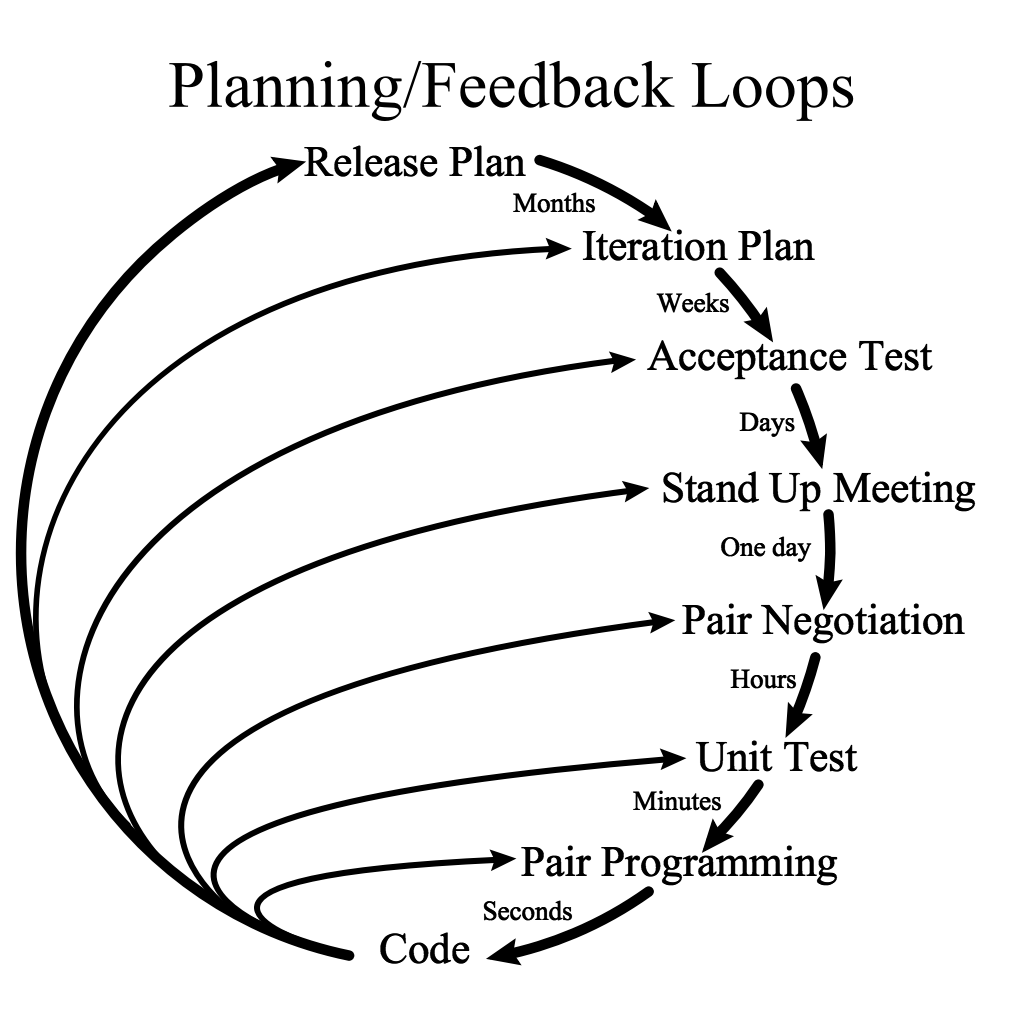
\includegraphics[scale=0.2]{diagrams/extreme_programming.png}
\caption{Extreme programming planning loops.}
\end{figure}

\subsection{GitLab}

This platform will be the main tool for version control of the source code and issue tracking of different tasks.

\subsubsection*{\texttt{git}}

All code projects (pipelines, service and website) will be stored in my personal projects space in \company's GitLab domain. Tasks and issue projects will be related to each project.
\\\\
Using \texttt{git}, the versions will be forked in branches, each branch will stand for an specific issue. \textit{Master} will be the main branch where the latest production version will be.

\subsubsection*{Tasks and issues}

The \textbf{issue tracking} will be very helpful in order to monitor the evolution of the project. Issues will be composed by a title, description, milestone, labels (if needed), due date and weight, and represents a new functionality. In order to know the status, issues will be listed in three columns:

\paragraph*{Backlog:}

Known tasks that haven been started yet. Could be a well defined task, with a very clear description, due date and weight, or just a draft.

\paragraph*{WIP:}

Work in Progress. The task is being considered, developed or tested.

\paragraph*{Done:}

Tasks finished, tested and done. Ready for production.

%----------------------------------
% CHAPTER 4: Requirements analysis
%----------------------------------

\chapter{Requirements analysis}

\label{chapter04}

%-----------------
%   SECTION 4.1
%-----------------

\section{Stakeholders}

Initially it seemed difficult to find stakeholders and actors in these project apart from the providers. It is not a tool for the user of \company.
\\\\
After talking with the squad lead and then the product owner of DeLorean a lot of stakeholders appeared: DeLorean squad, Marketing Automation squad, Data tribe, etc. Each of these stakeholders has different use cases and the project became very interesting for a considerable part of \company.

\subsection{DeLorean squad} \label{dlr}

DeLorean's Single Flight Number service, also known as \textit{Timetable SFN Service}, provides all the \textbf{current} flights. This is a little bit of a problem when trying to get historical data because Timetable SFN Service does not provide past flights information, it is always \textbf{up-to-date}. In order to get this data it is needed to go one step back in the whole DeLorean data processing: \textit{Timetable Pipeline}.
\\\\
The \thesis\ must look old versions of the file created by the \textit{Timetable Pipeline} to get older routes. Then, \squad\ is a \thesis\ stakeholder because it will be using its Pipeline's data.

\subsubsection*{Product Owner} \label{product_owner}

\textbf{Jen Agerton} is the Product Owner of DeLorean squad. She realized that the \thesis\ is very useful for other squads like \nameref{mas} and providers (air carrier companies). Apart from being the \squad\ product owner, she is also in charge of the negotiation with providers and airlines. The comparison of offer and demand is very useful to find user trends and can help airlines when scheduling flights.

\subsubsection*{DeLorean's squad Lead}

\textbf{Francisco López} and I had the initial idea for this project. He saw an opportunity for the future (after project's delivery) orienting the \thesis\ for Machine Learning purpose: The information that the comparison server provide is very useful for constructed routes\footnote{combination of two SFN }.
\\\\
Looking at the evolution of timetables and user demand, \squad\ could make some assumption when combining routes to create constructed routes.

\subsection{Marketing Automation squad} \label{mas}

Marketing Automation squad enables scalable growth by automating workflows, and the collection of insightful data. They have three main goals:

\begin{itemize}
  \item Provide data to support decision making
  \item Automated, data driven campaign management
  \item Budget process automation
\end{itemize}

The \thesis\ will be very useful for the first goal. The data provided by the comparison has high value in marketing decisions. Looking at historical data, \nameref{mas} could post an advertisement about trend routes in a specific time of the year.

\subsection{Data tribe}

In Data tribe, State Machine squad captures the user actions, so they know where the user gets stuck or if they finally reach the provider of the flight. Other squads like Clan A and Clan B just gets users queries in flights, hotels and car hiring. The second data source of the \thesis\ (user searches and queries) will be obtained from these squads.

\subsection{Other \company\ developers}

Last (in \company) but not least, a new service will appear in the company, all developers will be able to use it and build software using the \thesis's data. For instance, it can be used as a training for a complex Machine Learning\cite{machine_learning_coursera}.
\\\\
The server Application Program Interface, used by the Web UI to visualize all data, will be public inside \company. This and all the documentation will be very helpful for developers.

\subsection{OAG} \label{sh_oag}

OAG is a company that collects all logistic flights information. \squad\ reads data from them, it is the main provider of information regarding routes. They are the world's largest network of air travel data to provide accurate, timely, actionable digital information and applications to the world's airlines, airports, government agencies and travel-related service companies\cite{oag}.

\subsection{Providers} \label{providers}

In the future, providers could take profit from \thesis. Companies will be able to know which of their routes or airports work better with user tendencies, they will be able to improve the flights service and make it more efficient, reducing number of flights in \textit{non-profitable} routes. They will also know which are the best places to invest looking at \textit{over-requested} routes.

\subsection{Traveler}

\company users are one of the main sources of information. Without them, the comparison cannot be made. The results of the comparison can also help them, not directly, but if providers somehow manage flights and routes following the \thesis\ results, the traveler experience will improve.

%-----------------
%   SECTION 4.2
%-----------------

\section{Functional requirements}

\thesis\ has a lot of functional requirements, features or functionalities that define this software usage. 

\begin{enumerate}
    \item \textbf{Search availability values by origin, destination, month and year}: Let the user of the \thesis\ search available flights evolution by date, for a given route (origin and destination), month and year of the flight.
    \\
    \item \textbf{Search searches values by origin, destination, month and year}: Same as feature \#1, but for user searches instead of available flights.
    \\
    \item \textbf{Search multiple availability values}: Be able to search and show multiple availability values for different flights in the same chart, easing the comparison between both queries. For example: \textit{Route A-B in August 2018 shows more availability than route A-C in August 2018 from January to March, but A-C has more availability than A-B from April until today.}
    \\
    \item \textbf{Search multiple searches values}: Be able to query and display multiple user searches values for different routes in the same chart, easing the comparison between both queries. For example: \textit{Route A-B in August 2017 shows more searches than route A-B in December 2017 from January to June.}
    \\
    \item \textbf{Search multiple mixed values}: Enable comparison between availability and searches as well. Search and display the comparison in the chart.
    \\
    \item \textbf{Add new query to chart}: Search for offer or demand (features \#1 or \#2) and display the result in the chart.
    \\
    \item \textbf{Remove query from chart}: Remove data from the chart, stop displaying an specific query's data.
    \\
    \item \textbf{Historical data API}: Enable an endpoint where developers can get historical data for a given route, month, year and source (available flights and user searches).
\end{enumerate}

%-----------------
%   SECTION 4.3
%-----------------

\section{Non-functional requirements}

Apart from the features, the \thesis\ also need to satisfy other requirements in terms of usability, latency, precision and more.

\begin{enumerate}
    \item \textbf{Usability}: The final user will be focused on the data that the \thesis\ will serve, so the user cannot be distracted or annoyed by the website usage.
    \\
    \item \textbf{Time availability}: The data should be available at any time, 24 hours per day, 7 days a week.
    \\
    \item \textbf{Usage availability}: This tool must be only available for \company\ employees, for now; and providers that are interested and \company\ agreed to give them access. That is why the endpoint will only be accessible from \company\ VPN\cite{palo_alto_networks}.
    \\
    \item \textbf{Speed and latency}: The application will have a lot of data to show, but the the charts to load cannot take much time or the comparisons will be slow, maybe annoying and could confuse the user.
    \\
    \item \textbf{Reliability}: A loss in historical data can be catastrophic, users could make wrong decisions because of not reliable data.
    \\
    \item \textbf{Scalability}: Every day, the amount of data of the application increases by one million records at least. The system must be able to process all this data, store it and serve it with no problem and with any notable difference from the first day, until the last one.
    \\
    \item \textbf{Maintainability}: The code can adapt to changes easily, user searches and flights models may change in the future, the code must adapt to these changes.
\end{enumerate}

%-----------------
%   SECTION 4.4
%-----------------

\section{User stories}

Instead of use cases, the requirements will be defined by user stories. Usually use cases are more specific, but user stories often work better for agile development.
\\\\
Since a use case is a description of interactions between one or more actors and the application, a user story focus in what the customer will actually do with the system.
\\\\
User stories will follow the following format: \textit{As an [actor] I want [action] so that [achievement]}. Stories will also have an acceptance criteria, a list of conditions that must be fully satisfied in order to the story be completed.

\subsection*{Story \#1}

\begin{displayquote}
As a \nameref{mas} member I want to compare availability of two or more routes in a specific month so that I can guess which is the most common route to travel with airlines.
\end{displayquote}

\subsubsection*{Acceptance criteria}

\begin{enumerate}
    \item User can execute at least two queries in a Web UI.
    \item The website displays a line chart with the amount of flights available by date.
    \item The chart shows a clear difference between different queries.
    \item The user can remove or add new routes.
\end{enumerate}

\subsection*{Story \#2}

\begin{displayquote}
As a \nameref{mas} member I want to compare searches of two or more routes in a specific month so that I can guess which is the most desired route by travelers.
\end{displayquote}

\subsubsection*{Acceptance criteria}

\begin{enumerate}
    \item User can execute at least two queries in a Web UI.
    \item The website displays a line chart with the amount of searches by date.
    \item The chars shows a clear difference between different queries.
    \item The user can remove or add new routes.
\end{enumerate}

\subsection*{Story \#3}

\begin{displayquote}
As a \nameref{mas} member I want to compare availability and searches of one route in a specific month so that I can see if it is over-requested or non-profitable.
\end{displayquote}

\subsubsection*{Acceptance criteria}

\begin{enumerate}
    \item User can execute two queries in a Web UI.
    \item The website displays a line chart with different results.
    \item The chars shows a clear difference between availability query and demand query.
\end{enumerate}

\subsection*{Story \#4}

\begin{displayquote}
As a \company\ developer I want to get a big amount of historical data from flights availability so that I can develop complex Deep Learning software.
\end{displayquote}

\subsubsection*{Acceptance criteria}

\begin{enumerate}
    \item The developer has an API endpoint.
    \item The data structure is simple.
    \item The data has some well-known format.
\end{enumerate}

\subsection*{Story \#5}

\begin{displayquote}
As a \company\ developer I want to get a big amount of historical data from user searches so that I can develop complex Deep Learning software.
\end{displayquote}

\subsubsection*{Acceptance criteria}

\begin{enumerate}
    \item The developer has an API endpoint.
    \item The data structure is simple.
    \item The data has some well-known format.
\end{enumerate}

\subsection*{Story \#6}

\begin{displayquote}
As a airline provider of \company\ I want to see the evolution of demand so that I can schedule flights properly depending on user demand.
\end{displayquote}

\subsubsection*{Acceptance criteria}

\begin{enumerate}
    \item The website shows data readable for humans.
    \item The data is displayed by date.
    \item The user knows what he/she is seeing.
\end{enumerate}



%----------------------------------
% CHAPTER 5: Requirements analysis
%----------------------------------

\chapter{Specification}

\label{chapter05}

As explained before, the \thesis\ is a big data problem, but in order to this amount of data be useful and make actual sense, the data model must be correct and very well defined. If there is some conceptual mistake the data displayed in the charts will not be reliable, so it will not be satisfying non-functional requirement of reliability (\#5).
\\\\
The data model must be also subject to change and pretty clear, to fulfill non-functional requirement of Maintainability (\#7).

%-----------------
%   SECTION 5.1
%-----------------

\section{Routes model}

\squad's pipeline, writes the data in \textbf{Single Flight Number} model. This model is not useful for this project because of the \nameref{sfn-date-set} schema. The timetable pipeline can also write following the \textbf{unified timetable} schema, this model presents the final master set of single flight number timetables that have been merged and de-duplicated from multiple sources. Dates schema are compatible with the \thesis\ purpose.

\subsection{Single Flight Number Object Model} \label{sfn-model}

The \textbf{Single Flight Number} (SFN) timetables data schema is designed with the following object model.

\subsubsection*{SFN Route}

Represents a route between 2 airports and the SFNs timetable that are available on that route. It is composed by three fields:

\begin{table}[H]
\centering
\begin{tabular}{|>{\raggedright\arraybackslash}p{2.5cm}|>{\raggedright\arraybackslash}p{4cm}|>{\raggedright\arraybackslash}p{2.5cm}|>{\raggedright\arraybackslash}p{2cm}|>{\raggedright\arraybackslash}p{1.2cm}|}
\hline
\textbf{Field}       & \textbf{Description}                                 & \textbf{Data Type}           & \textbf{Required} & \textbf{Key} \\ \hline
\textbf{Origin}      & The origin airport or station for the timetable      & Integer                      & Yes               & Yes          \\ \hline
\textbf{Destination} & The destination airport or station for the timetable & Integer                      & Yes               & Yes          \\ \hline
\textbf{Series}      & The SFN timetables associated with the route         & List of SFN Timetable Series & Yes               & No           \\ \hline
\end{tabular}
\caption{Single Flight Number Route fields}
\label{sfn-route}
\end{table}

\subsubsection*{SFN Timetable Series}

Represents a SFN timetable for the year ahead.

\begin{table}[H]
\centering
\begin{tabular}{|>{\raggedright\arraybackslash}p{2.5cm}|>{\raggedright\arraybackslash}p{4cm}|>{\raggedright\arraybackslash}p{2.5cm}|>{\raggedright\arraybackslash}p{2cm}|>{\raggedright\arraybackslash}p{1.2cm}|}
\hline
\textbf{Field}                           & \textbf{Description}                              & \textbf{Data Type}      & \textbf{Required} & \textbf{Key} \\ \hline
\textbf{Marketing Carrier}               & The ID of the carrier that is marketing the flight & Integer                 & Yes               & Yes          \\ \hline
\textbf{Marketing Carrier Flight Number} & The flight code assigned by the marketing carrier  & Integer                 & Yes               & Yes          \\ \hline
\textbf{Series Items}                    & 1..n Series Items                                  & List of SFN Series Item & Yes               & No           \\ \hline
\end{tabular}
\caption{Single Flight Number Timetable Series fields}
\label{sfn-series}
\end{table}

\subsubsection*{SFN Timetable Series Item}

A Timetable Series Item represents a specific configurations of operating carrier, stops and times of day for a given SFN timetable. For example for a given Marketing Carrier / Flight Number, the Operating Carrier or times of day may change through the year.

\begin{table}[H]
\centering
\begin{tabular}{|>{\raggedright\arraybackslash}p{2.5cm}|>{\raggedright\arraybackslash}p{4cm}|>{\raggedright\arraybackslash}p{2.5cm}|>{\raggedright\arraybackslash}p{2cm}|>{\raggedright\arraybackslash}p{1.2cm}|}
\hline
\textbf{Field}                           & \textbf{Description}                                                                           & \textbf{Data Type}            & \textbf{Required} & \textbf{Key} \\ \hline
\textbf{Operating Carrier}               & The ID of the administrating operating Carrier                                                 & Integer                       & Yes               & Yes          \\ \hline
\textbf{Operating Carrier Flight Number} & The flight code assigned by the administrating operating carrier                               & Integer                       & No                & No           \\ \hline
\textbf{Physical Operating Carrier}      & The ID of the 'physical' operating Carrier                                                     & Integer                       & Yes               & Yes          \\ \hline
\textbf{Stop Count}                      & The total number of stops (can be derived from the list of stops)                              & Integer                       & Yes               & No           \\ \hline
\textbf{Stops}                           & A list of via airports                                                                         & List of Integer               & No                & Yes          \\ \hline
\textbf{Departure time}                  & The time of departure in the current time zone of the origin station (minutes after 00:00)     & Integer                       & Yes               & Yes          \\ \hline
\textbf{Arrival time}                    & The time of arrival in the current time zone of the destination station (minutes after 00:00)  & Integer                       & Yes               & Yes          \\ \hline
\textbf{Arrival day offset}              & The number of days after the departure date that the flight arrives                            & Integer                       & Yes               & Yes          \\ \hline
\textbf{Duration}                        & The total flight duration (can be derived from the departure and arrival times and day offset) & Integer                       & Yes               & No           \\ \hline
\textbf{Traffic Restrictions}            & Restrictions relating to how a flight can be sold                                              & Traffic Restrictions instance & Yes               & Yes          \\ \hline
\textbf{DateSets}                        & The dates that this Timetable Series Item is flown                                             & Array of DateSet              & Yes               & No           \\ \hline
\end{tabular}
\caption{Single Flight Number Timetable Series Item fields}
\label{sfn-series-item}
\end{table}

\subsubsection*{Traffic restrictions}

A set of flags indicating restrictions relating to how an timetabled flight might be sold. Not relevant for this project.

\subsubsection*{SFN Date Set} \label{sfn-date-set}

A Date Set represents a start date and day of week pattern for a given Timetable Series Item.

\begin{table}[H]
\centering
\begin{tabular}{|>{\raggedright\arraybackslash}p{2.5cm}|>{\raggedright\arraybackslash}p{5.2cm}|>{\raggedright\arraybackslash}p{2.5cm}|>{\raggedright\arraybackslash}p{2cm}|}
\hline
\textbf{Field}        & \textbf{Description}                                                                                  & \textbf{Data Type}              & \textbf{Required} \\ \hline
\textbf{Start Date}   & The start date that this set is applicable from                                                       & String (date format YYYY-MM-DD) & Yes               \\ \hline
\textbf{Data Sources} & The source(s) of the timetable data                                                                   & Array of sources (Enun)         & Yes               \\ \hline
\textbf{Availability} & A set of offsets indicating the dates that the associated series is available (up to 13 months ahead) & Array of week days (Enum)       & Yes               \\ \hline
\end{tabular}
\caption{Single Flight Number Timetable Date set fields}
\label{sfn-date-set}
\end{table}

Since the dates are represented by week days as an enumeration (\textit{mon}, \textit{tue}, \textit{wed}, ...), the grouping of flights by \textbf{day} or \textbf{month}\footnote{In version X the model changes and the pipelines group by month} becomes very difficult and non trivial. That is why the \thesis\ uses the \textbf{Unified} model.

\subsection{Unified Timetable Object Model} \label{unified-model}

In the timetable pipeline owned by \squad\ first maps all data to Unified model then it is mapped to the final Single Flight Number Timetable model. Unified model is very similar than \nameref{sfn-model}, it uses \textbf{Airport object} instead of an integer and a set of strings in date format \texttt{YYYY-MM-DD} in date sets, availability:

\begin{figure}[H]
\centering
\includegraphics[scale=0.6]{diagrams/unified_model.png}
\caption{Unified Timetables UML class diagram}
\label{unified-uml}
\end{figure}

With this model, the \nameref{flights-offer-pipeline} can apply flattening and grouping easily into this model.
\\\\
Airport's code will be used to identify them and pairs of codes will represent a route. This code is also know as IATA Code\cite{iata_code}.

%-----------------
%   SECTION 5.2
%-----------------

\section{Searches model}

The user searches are stored in a huge database that contains flight search, car hire search and hotel search, one has value an the other two are \texttt{null}.

\begin{figure}[H]
\centering
\includegraphics[scale=0.6]{diagrams/flight_search.png}
\caption{Flight search UML class diagram}
\end{figure}

A user query in \company\ contains a lot of information, but most of it is not useful for the purpose of this project.

%-----------------
%   SECTION 5.3
%-----------------

\section{Flight Availability Model}

As we can see above in the \nameref{unified-model}, flights are grouped by routes, then by flights, series and finally we reach the date. The \thesis\ will be queried by route and date, so it is important to have the flights stored and count its availability at date level.
\\\\
The flights availability records will be grouped by route and then by date.

\begin{figure}[H]
\centering
\includegraphics[scale=0.6]{diagrams/flights_availability_model.png}
\caption{Flights Availability UML class diagram}
\end{figure}

Flights Availability and \nameref{unified-uml} looks very similar. The main difference is that a route in Unified model contains a set of flights but a set of dates in Flight Availability.
\\\\
Date class contains a strings in date format \texttt{YYYY-MM-DD} and the number of available flights on that date. This last field is the same as the size of the set of flights it is composed by. The flight availability model has \textbf{a lot of duplicated values}, one flight operates a lot of dates and it is grouped by date\footnote{All flights data transformations explained in \nameref{fop-data-transformations}}.

%-----------------
%   SECTION 5.4
%-----------------

\section{User Searches Model}

The user searches model has been simplified and a lot of fields from the original model has been removed. Since the amount of data of user searches increases on the order of millions per day, the model contains the basic data.

\subsubsection*{User Searches Route}

\begin{table}[H]
\centering
\begin{tabular}{|>{\raggedright\arraybackslash}p{2.5cm}|>{\raggedright\arraybackslash}p{4cm}|>{\raggedright\arraybackslash}p{2.5cm}|>{\raggedright\arraybackslash}p{2cm}|>{\raggedright\arraybackslash}p{1.2cm}|}
\hline
\textbf{Field}       & \textbf{Description}                         & \textbf{Data Type}     & \textbf{Required} & \textbf{Key} \\ \hline
\textbf{Origin}      & The origin airport or station IATA code      & String                 & Yes               & Yes          \\ \hline
\textbf{Destination} & The destination airport or station IATA code & String                 & Yes               & Yes          \\ \hline
\textbf{Dates}       & The SFN timetables associated with the route & List of Searches Dates & Yes               & No           \\ \hline
\end{tabular}
\caption{User Searches Route fields}
\end{table}

\subsubsection*{Searches Date}

\begin{table}[H]
\centering
\begin{tabular}{|>{\raggedright\arraybackslash}p{2.5cm}|>{\raggedright\arraybackslash}p{4cm}|>{\raggedright\arraybackslash}p{2.5cm}|>{\raggedright\arraybackslash}p{2cm}|>{\raggedright\arraybackslash}p{1.2cm}|}
\hline
\textbf{Field} & \textbf{Description}                           & \textbf{Data Type} & \textbf{Required} & \textbf{Key} \\ \hline
\textbf{Date}  & Date for the leg that was searched             & String             & Yes               & Yes          \\ \hline
\textbf{Count} & Number of searches for that route in that date & Integer            & Yes               & No           \\ \hline
\end{tabular}
\caption{Searches Date fields}
\end{table}








%-------------------
% CHAPTER 6: Design
%-------------------

\chapter{Design}

\label{chapter06}

With all the specification of the data the \thesis\ will work with, a good architecture for the system is needed. The whole software project is split in four different parts: Available Flights Pipeline, User Searches Pipeline, Comparison Service and Web UI.
\\\\
In this chapter all four architectures for the four different parts will be defined and analyzed. All alternatives will also be defined and explain why are not in the final architecture.
\\\\
Even so, first it is good to understand the general architecture of the whole \thesis.

%-----------------
%   SECTION 6.1
%-----------------

\section{Architecture}

The \thesis\ is split in very notable three layers: Data collection and processing, Comparison Server and Web UI. Two of this layer, server and user interface, suit exactly two of the four remarkable in the whole system, the Comparison Service and Web UI. Named the same to avoid confusion.
\\\\
An important characteristic of the \thesis\ is that the only way to feed the database is from the data collection and processing layer. This is different of most of projects and examples I have worked before in the University.
\\\\
The most common architecture used is a three layers (data layer, domain layer and presentation layer) where in the presentation layer the user could usually put data into the data layer. The \thesis\ work very different: The user interface (that is the presentation layer) does not put or modifies any data from the database. It only reads. The only way the database can be filled with valid data is from the \textit{data collection and processing layer}.

\begin{figure}[H]
\centering
\includegraphics[scale=0.7]{diagrams/architecture01.png}
\caption{General view of the \thesis\ architecture.}
\end{figure}

% SUB SECTION 6.1.1

\subsection{Data collection and processing} \label{data_layer}

This layer is composed by two components, one for each data processing: Available Flights Pipeline and User Searches Pipeline. The purpose of this layer is to collect all data necessary to do the comparison and filter and group according the final data model needed.
\\\\
Both components in the this layer uses very similar technologies and are written in Scala\nameref{scala}. The data is read from different sources that already exist in \company\ and have a well defined design (\nameref{data_tribe} and \squad's pipeline) and amazon web services (\nameref{athena} and \nameref{s3}, S3). The whole data processing or data pipeline ran in Apache Spark, in an \nameref{emr} cluster. In the end of the process both pipelines write into the same Storage service.

\begin{figure}[H]
\centering
\includegraphics[scale=0.7]{diagrams/architecture-data.png}
\caption{General view of the data collection and processing layer's architecture.}
\end{figure}

\subsubsection*{Amazon Athena} \label{athena}

\begin{figure}[H]
\centering
\includegraphics[scale=0.1]{resources/athena-logo.png}
\caption{Amazon Athena logo}
\end{figure}

Amazon Athena\cite{athena}, is an Amazon Web Service that lets query data stored in \nameref{s3} (S3) using standard SQL\cite{sql}. It have no server running, so it have no infrastructure to manage.
\\\\
To access the data, Athena simply points to an S3 bucket with a defined schema and it lets you query its data with SQL queries. The cost of the service is based on the queries you run.
\\\\
\nameref{data_tribe} is responsible of creating schemas for Athena to read S3 buckets. They have a huge bucket called \texttt{grappler\_master\_archive} that contains all the user searches. Athena is now the easiest way to access user searches data.

\subsubsection*{Amazon Simple Storage Service} \label{s3}

\begin{figure}[H]
\centering
\includegraphics[scale=0.1]{resources/s3-logo.png}
\caption{Amazon Simple Storage Service logo}
\end{figure}

Amazon Simple Storage Service\cite{s3}, also known as \textit{S3}, stores data as objects within resources called buckets. It allows store unlimited objects in a bucket, also write, read and delete those objects. The maximum size of these objects is 5 terabytes. The access permission to buckets can be controlled its configuration.
\\
In \company, most of the results of \nameref{data_pipeline}s are stored as a single or multiple files in S3, then those are processed by \nameref{lambda} functions or other services. \squad\ stores timetables as a JSON\cite{json} file in its S3 bucket. Data tribe has also a bucket for user searches (and much more) data, but, as explained before, it provides access from \nameref{athena}.

\subsubsection*{Apache Spark\textsuperscript{TM}} \label{apache_spark}

\begin{figure}[H]
\centering
\includegraphics[scale=0.1]{resources/apache-spark_logo.png}
\caption{Apache Spark\textsuperscript{TM} logo}
\end{figure}

Apache Spark\textsuperscript{TM} is a unified analytics engine for large-scale data processing. It was created and it is currently maintained by the Apache Software Foundation\cite{apache_software_foundation}.
\\\\
Is one of the most popular fast and general-purpose cluster computing systems. It can run in a lot of different environments, Apache\textsuperscript{TM} Hadoop\textregistered\cite{hadoop}, Kubernetes\cite{k8s}, \nameref{emr} and much more. Spark provides four APIs: Java, Scala, Python, R and SQL. Over 80 high-level operators can help building parallel processes and can be called from most of its APIs. Both data pipelines are written using the Scala API.
\\\\
Apache Spark\textsuperscript{TM}'s architecture is based in \textit{Resilient Distributed Datasets}, RDD, a read-only multiset distributed in multiple machines. Those machines are based in the MapReduce paradigm, a programming model for big data dumps processing. Since the data is distributed, this process runs in parallel.
\\\\
To an RDD, you can apply two kind of operations: transformations and actions:
\\\\
A \textbf{Spark Transformation} are functions that creates a new RDD form an existing one. Transformations are lazy operations and only are executed when an action is called. When calling a transformation, a link is created between two RDDs, this happens successively until the action is executed. Then, all transformations are applied until the action. These links between transformations are edges in the Apache Spark\textsuperscript{TM}'s Directed Acyclic Graph.

\begin{figure}[H]
\centering
\includegraphics[scale=0.3]{resources/dag.png}
\caption{Example of a Directed Acyclic Graph (DAG).}
\end{figure}

Most common transformations used in the project are:

\begin{displayquote}
\texttt{def map[R](f: Function[T, R]): RDD[R]}
\\
Return a new RDD by applying a function to all elements of this RDD.
\\\\
\texttt{def flatMap[U](f: FlatMapFunction[T, U]): RDD[U]}
\\
Return a new RDD by first applying a function to all elements of this RDD, and then flattening the results.
\\\\
\texttt{def filter(f: Function[T, Boolean]): RDD[T]}
\\
Return a new RDD containing only the elements that satisfy a predicate.
\\\\
\texttt{def groupBy[U](f: Function[T, U]): PairRDD[U, Iterable[T]]}
\\
Return an RDD of grouped elements. Each group consists of a key and a sequence of elements mapping to that key.
\end{displayquote}

A \textbf{Spark Action} are RDD operations that do not return an RDD-like value. Actions are executed when called, first running all transformation in the directed acyclic graph of transformations.
\\\\
Most common actions used in pipelines are:

\begin{displayquote}
\texttt{def count(): Long}
\\
Return the number of elements in the RDD.
\\\\
\texttt{def fold(zeroValue: T)(f: Function2[T, T, T]): T}
\\
Aggregate the elements of each partition, and then the results for all the partitions, using a given associative function and a neutral "zero value".
\\\\
\texttt{def foreach(f: VoidFunction[T]): Unit}
\\
Applies a function f for all elements of this RDD.
\end{displayquote}

\subsubsection*{Amazon Data Pipeline} \label{data_pipeline}

\begin{figure}[H]
\centering
\includegraphics[scale=0.1]{resources/data_pipeline-logo.png}
\caption{Amazon Data Pipeline logo}
\end{figure}

Amazon Data Pipeline\cite{data_pipeline} service helps running processes reliably and move data between Amazon Web Services Storage services. In the \thesis\ it is used to move data from \nameref{athena} or \nameref{s3} to \nameref{emr} and from \nameref{emr} back to \nameref{s3}.
\\\\
If, for any reason, the pipeline fails, this service retries the execution, if the execution fails constantly, the data pipeline stops and sends a failure notification to the owner.
\\\\
Data Pipelines can also be scheduled to run every hour, every two hours, every day, week, etc. Both pipelines are scheduled to run once a day every day. In every executions, first builds the environment (\nameref{emr} and \nameref{apache_spark}) and then runs the JAR\cite{jar} file generated from available flights pipeline and user searches pipeline. To avoid unnecessary dependencies, there are two \nameref{data_pipeline}s, one for the flights and another for the user searches.

\subsubsection*{Amazon Elastic MapReduce} \label{emr}

\begin{figure}[H]
\centering
\includegraphics[scale=0.1]{resources/emr-logo.png}
\caption{Amazon Elastic MapReduce logo}
\end{figure}

Amazon Elastic MapReduce\cite{emr} (EMR) provides a Hadoop\cite{hadoop} framework that makes easy, fast, and cost-effective to process vast amounts of data. As explained before, \nameref{apache_spark} runs in Hadoop. These clusters are prefect for running big data applications and pipelines.
\\\\
EMRs use master/slave communication model. This, applied to \nameref{apache_spark}, means that one cluster divides the data and does the partition of the RDDs while the rest of the instances, the slaves, execute the actions and transformations.
\\\\
The EMR configuration for each pipeline will be:

\begin{table}[H]
\centering
\begin{tabular}{|p{5cm}|p{5cm}|p{3cm}|}
\hline
\textbf{Field}                        & \textbf{Description}         & \textbf{Value}      \\ \hline
\textbf{Release}                      & EMR version                  & \texttt{emr-5.12.0} \\ \hline
\textbf{Cluster master instance type} & Instance type of the master  & \texttt{m3.xlarge}  \\ \hline
\textbf{Cluster core instance type}   & Instance type of the slaves  & \texttt{m3.xlarge}  \\ \hline
\textbf{Cluster size}                 & Number of slaves clusters    & 6                   \\ \hline
\textbf{Timeout}                      & Insurance to not run forever & 5 hours             \\ \hline
\end{tabular}
\caption{EMR configuration}
\end{table}

EMR 5.12.x was the latest version when the project started. Newer versions does not have any relevant upgrade.
\\\\
\texttt{m3.xlarge} has the following hardware specs:

\begin{table}[H]
\centering
\begin{tabular}{|p{3.5cm}|p{2cm}|p{1.5cm}|p{1.5cm}|p{3.5cm}|}
\hline
\textbf{Name}                  & \textbf{API Name}  & \textbf{Memory} & \textbf{vCPUs} & \textbf{Instance Storage}    \\ \hline
M3 General Purpose Extra Large & \texttt{m3.xlarge} & 15.0 GiB        & 4              & 80 GiB (\(2 \times 40\) GiB) \\ \hline
\end{tabular}
\caption{\texttt{m3.xlarge} specs}
\end{table}

% SUB SECTION 6.1.2

\subsection{Service} \label{service}

The service is the middle layer of the \thesis. A simple Python\cite{python} service reads data written by the components in the \nameref{data_layer} layer and serves the data through an \nameref{ecs}.
% using Boto3\footnote{Boto\cite{boto3} is the Amazon Web Services (AWS) SDK for Python} 
\\\\
A \nameref{docker} container is created and managed by \nameref{ecs}. In this container the Python\cite{python} service is deployed.
% with AIOHTTP\footnote{AIOHTTP\cite{aiohttp} is an Asynchronous HTTP Client/Server library for Python. Perfect for HTTP Servers.} 

% \begin{figure}[H]
% \centering
% \includegraphics[scale=0.7]{diagrams/architecture-service.png}
% \caption{General view of the web service layer's architecture}
% \end{figure}

\subsubsection*{Amazon Elastic Container Service} \label{ecs}

\begin{figure}[H]
\centering
\includegraphics[scale=0.1]{resources/ecs-logo.png}
\caption{Amazon Elastic Container Service logo}
\end{figure}

Amazon Elastic Container Service, also known as ECS\cite{ecs}, is a container management service that supports \nameref{docker}. It ease the container orchestration with a simple API.

\subsubsection*{Docker} \label{docker}

\begin{figure}[H]
\centering
\includegraphics[scale=0.1]{resources/docker-logo.png}
\caption{Docker logo}
\end{figure}

Docker\cite{docker} is tool that creates a container where you can run whichever application you want with its environment. A Docker container can be created in a lot of machines, for example in an \nameref{ecs}.

% SUB SECTION 6.1.3

\subsection{Website}

Finally, the presentation layer gets data from the \nameref{service} and displays. The architecture of this layer is very simple, the website does an HTTP request to the service and gets a JSON back.
\\\\
It is also ran in a \nameref{docker} container deployed in \nameref{ecs}.

%-----------------
%   SECTION 6.2
%-----------------

\section{Components}

Once the technology each layer will use is set, lets define the code architecture of each component.

% SUB SECTION 6.2.1

\subsection{Available Flights Pipeline} \label{available-flights-pipeline}

The flight offer data pipeline reads timetables from \squad's ingest pipeline, stored in \nameref{unified-model} and group, map and filter to \nameref{flight-availablity-model}.
\\\\
\squad's Ingest Pipeline writes all the timetables in its \nameref{s3} bucket in very JSON\cite{json} alike format. \nameref{apache_spark} and the components of \squad\ that read routes from the result file line by line, each of those lines is a Unified Route. Luckily when Apache Spark reads a file i creates an RDD of Strings, one record per line; so when reading \squad's file, it will get an RDD of Unified Routes in JSON\cite{json} format.
\\\\
For all data processing, the pipeline is split in well-defined stages. Each stage is a \textbf{Singleton}\footnote{Design pattern explained in \nameref{appendix_b} on page \pageref{appendix_b}.} object: This pattern ensures a class only has one instance, and provides a global point of access to it.
\\\\
All stages have a name to be identified and a function \texttt{run} that executes the Spark transformations and actions needed to complete its purpose. The Available Flights Pipeline is composed by six stages grouped in two \textit{sub-pipelines}:

\subsubsection*{Routes \textit{sub-pipeline}}

This \textit{sub-pipeline} basically regroup Unified Routes data to a friendly model for the Routes Availability. It does not discards any field just in case those want to be used for future features, improvements or applications.

\begin{itemize}
    \item \textbf{Read Routes stage}: It reads the \texttt{version.txt} file from \squad's bucket, there it get the latest version of the timetables and read them, returning an Strings RDD.
    \item \textbf{JSON to Route stage}: Maps from a String RDD to a Unified Route Class using \nameref{gson}.
    \item \textbf{Flights Flattening stage}: Flats all routes' series at date level, duplicating origins and destinations of flights that have the same route. There are three flattening, from series to series item, from series item to date sets and finally from date sets to single dates. Going from 64,000 routes to 75,000,000 flights. The amount of data increases a lot in this point.
    \item \textbf{Group Routes stage}: After flattening at date level, flights are grouped by date. There is a lot of shuffling\footnote{Sharing data between different nodes or machines} which makes it a slow process.
\end{itemize}

Apart from these four stages, it has other to parse grouped routes by date objects to JSON\cite{json} and another to write it to \nameref{s3}, but those are not necessary, both stages are disabled.

\subsubsection*{Summary \textit{sub-pipeline}}


\begin{itemize}
    \item \textbf{Map Summary stage}: Discards lots of fields from the model resulting from the routes \textit{sub-pipeline} and maps the data to the final records that will be written in the database.
    \item \textbf{Write Records stage}: Writes into \nameref{s3} using \nameref{scala_aws}.
\end{itemize}

\begin{figure}[H]
\centering
\includegraphics[scale=0.45]{diagrams/available-flights-pipeline-architecture.png}
\caption{Available flights pipeline architecture and data flow diagram}
\end{figure}

To end up doing this architecture, there have been a lot of alternatives during all the development of the Available Flights Pipeline.

\subsubsection*{Amazon Relational Database Service} \label{rds}

\begin{figure}[H]
\centering
\includegraphics[scale=0.1]{resources/rds-logo.png}
\caption{Amazon Relational Database Service logo}
\end{figure}

In the beginning, the idea was to write all data to Amazon RDS, Relational Database Service\cite{rds}. This service offers a relational database in the cloud that can be accessed very fast. But there are two important reasons thy this option has been discarded:

\begin{itemize}
    \item \textbf{Cost}: It is very expensive to have an RDS active all the time. Some squads in \company\ use \nameref{rds} but only active some time a week for very specific purposes.
    \item \textbf{Knowledge}: I know about some squads that used that in some occasion, but not based in Barcelona. Reading some documentations and examples, it looked very difficult to set up and use, there were alternatives 
\end{itemize}

\subsubsection*{Amazon DynamoDB} \label{dynamodb}

\begin{figure}[H]
\centering
\includegraphics[scale=0.2]{resources/dynamodb-logo.png}
\caption{Amazon DynamoDB logo}
\end{figure}

Another idea about the database where the pipeline could write was Amazon RDS, Relational Database Service\cite{dynamodb}. This service offers a non-relational database in the cloud that can be accessed very fast. But there was one important reasons thy this alternative was discarded: The \textbf{Cost}, it is very expensive to have an DynamoDB, even more expensive than \nameref{rds}.
\\\\
Having this in mind, after some brainstorming, the final solution was found:

\subsubsection*{S3 and dates at month level} \label{month_version}

The main problem of this pipeline, that happens in the \nameref{user-searches-pipeline} as well, is that \textbf{versions are written every day} and does not delete anything. So it satisfies the functional requirement of Historical data (\#8)
\\\\
\squad\ provides flights for one year ahead and every day the data is uploaded in a new file to S3, the \nameref{available-flights-pipeline} reads this file and gets all flights for all days in the next year and writes them to the Database. It would be very easy for the service then read with an SQL table like:

\begin{table}[H]
\centering
\begin{tabular}{|p{2.5cm}|p{2.5cm}|p{3cm}|p{3cm}|p{2.5cm}|p{2.5cm}|p{1cm}|}
\hline
\texttt{origin}       & \texttt{destination}   & \texttt{version\_date}       & \texttt{flight\_date}        & \texttt{count}       \\ \hline
BCN                   & LGW                    & 2018-06-13                   & 2018-08-20                   & 14                   \\ \hline
BCN                   & LGW                    & 2018-06-13                   & 2018-08-21                   & 12                   \\ \hline
BCN                   & MAD                    & 2018-06-13                   & 2018-08-20                   & 34                   \\ \hline
\cellcolor{blue!5}BCN & \cellcolor{blue!5}EDI  & \cellcolor{blue!5}2018-06-13 & \cellcolor{blue!5}2018-08-12 & \cellcolor{blue!5}20 \\ \hline
\cellcolor{blue!5}BCN & \cellcolor{blue!5}EDI  & \cellcolor{blue!5}2018-06-14 & \cellcolor{blue!5}2018-08-12 & \cellcolor{blue!5}20 \\ \hline
\cellcolor{blue!5}BCN & \cellcolor{blue!5}EDI  & \cellcolor{blue!5}2018-06-15 & \cellcolor{blue!5}2018-08-12 & \cellcolor{blue!5}30 \\ \hline
BCN                   & EDI                    & 2018-06-15                   & 2018-09-14                   & 25                   \\ \hline
...                   & ...                    & ...                          & ...                          & ...                  \\ \hline
\end{tabular}
\caption{Snapshot example of service database table}
\end{table}

So, for instance, if the user queries for the evolution of the flights available from Barcelona to Edinburgh on August 12 of 2018, the service could simple run an SQL query to the Database like \texttt{SELECT * FROM flight\_availability WHERE origin = "BCN" AND destination = "EDI" AND flight\_date = "2018-08-12"}. Then the service could map the result to the desired schema and response it back to the client.
\\\\
Looks easy and simple, but the problem is that, as explained before, \nameref{rds} is very expensive. The only storage service left that does not take much time to develop is \nameref{s3}.
\\\\
Is very fast to write to S3, the whole data dump with more than 75 million flights can be written in less than a minute in a \textbf{single file}, but how about the reading from the service? Boto\footnote{Boto is the Amazon Web Services (AWS) SDK for Python, explained in \nameref{boto3} on page \pageref{boto3}} takes more or less an eighth of a second to access the file and more or less a quarter second to read the whole file. This is fine if the service just needs to read one file, but as explained before, the pipeline writes one file every day. So, for one query, in the worst case scenario, there are 365 files to open and read (days in one year). In other words, more than 4 minutes for the service to response a query. This does not satisfy the fourth non-functional requirement of Speed and Latency.
\\\\
The solution was to write one file per record, and inside it all the data about the flights for that route in that date. That way, \nameref{boto3} could run the \texttt{list\_bucket} function, that list all objects under the given key. This key, must contain the basic model's information:
\texttt{\$ORIGIN-\$DESTINATION/ \$DATE/ \$VERSION\_DATE-\$COUNT.json}

\break

\begin{verbatim}
BCN-LGW/
        2018-08-20/
                   2018-06-13-14.json
        2018-08-21/
                   2018-06-13-12.json

BCN-MAD/
        2018-08-20/
                   2018-06-13-34.json

BCN-EDI/
        2018-08-12/
                   2018-06-13-20.json
                   2018-06-13-20.json
                   2018-06-13-30.json
        2018-09-14/
                   2018-06-15-25.json
\end{verbatim}

The problem with this implementation, is that there are 75 million different records to write. It would take more than one day for the pipeline to write the whole data, very slow and expensive because of the EMR cluster running time.
\\\\
After analyzing the data, one solution was to only write changes, so there are no that big amount of files to write, but it was discarded because user searches change every day, not like flights, and the same problem would happen when writing in the other pipeline.
\\\\
Finally, checking the user stories and the purpose of this tool, a final decision was made: Data was going to be store that way, one record per day, but the number of records will be reduced \textbf{grouping flights by months} instead of having them by day. The final S3 directory structure would be:

\begin{verbatim}
BCN-LGW/
        2018-08/
                2018-06-13-26.json

BCN-MAD/
        2018-08/
                2018-06-13-34.json

BCN-EDI/
        2018-08/
                2018-06-13-20.json
                2018-06-13-20.json
                2018-06-13-30.json
        2018-09/
                2018-06-15-25.json
\end{verbatim}

With this design, the service takes less than a second to get all the data and the pipeline takes one hour to write all the records.

% SUB SECTION 6.2.2

\subsection{User Searches Pipeline} \label{user-searches-pipeline}

The user demand is obtained from \textbf{user searches} table in \nameref{athena}. Then the results of the Athena query are mapped to the same data model of the stored in S3 by the \nameref{available-flights-pipeline}.
\\\\
The first problem found in this pipeline was that the results from Athena were stored in a CSV\cite{csv} in S3, each row had a record with a format similar to JSON\cite{json}. Those records could not be parsed to an object using any library. Using RegEx\cite{regex} applied to rows treated as a String, the result were obtained.
\\\\
Another problem found is that as more data you request, more time it gets to finish the query, and it is not a lineal progression. To solve that, the query was split in four sub-queries. Four that request all user flight searches in hour ranges 00:00-05:59, 06:00-11:59, 12:00-17:59 and 18:00-23:59. Usually the resultant files take \textbf{30 gigabytes} in total.
\\\\
\nameref{user-searches-pipeline} is not split in \textit{sub-pipelines}. It has four stages in total:

\begin{itemize}
    \item \textbf{Athena Reader stage}: Queries Athena for user searches. Athena writes automatically to S3 and returns the file name. Four executions, one per hour range.
    \item \textbf{S3 Reader stage}: Gets the file name of the query result and reads it. CSV\cite{csv} to String RDD. Four executions too, one per file.
    \item \textbf{Search Query stage}: Gets the records from the Athena records, filters them by kind of search an other parameters, maps each record to the desired model and groups by route.
    \item \textbf{Write Records stage}: Writes into \nameref{s3} using \nameref{scala_aws}.
\end{itemize}

\begin{figure}[H]
\centering
\includegraphics[scale=0.45]{diagrams/user-searches-pipeline-architecture.png}
\caption{User searches pipeline architecture and data flow diagram.}
\end{figure}

% SUB SECTION 6.2.3

\subsection{Comparison Service} \label{comparison_service}

Once all the data is processed every day and stored into \nameref{s3}, it has to be served in an HTTP\cite{http} API.
\\\\
The Comparison Servie's API provides two endpoints, one for the comparison and another one for a single source request (flights or searches)\footnote{The \textit{environment} field can be \texttt{sandbox} or \texttt{prod}. Learn more about those environments in section \nameref{environments} on page \pageref{environments}.}. The main class, API Handler, execute a function when the endpoint is queried and uses an AWS Adapter that is directly connected to \nameref{boto3}. The API Handler returns a set of records in JSON format.
\\\\
The \textbf{Adapter}\footnote{Design pattern explained in \nameref{appendix_b} on page \pageref{appendix_b}.} converts the \nameref{boto3} interface into another interface that the API Handler expects. Adapter lets both classes work together that could not otherwise because of incompatible interfaces.

\begin{figure}[H]
\centering
\includegraphics[scale=0.5]{diagrams/server-architecture.png}
\caption{Comparison service class diagram.}
\end{figure}

\textbf{\texttt{/api/comparison/{environment}/{route}/{date}}}
\\\\
GET two sets of data for a given route and date: All existent versions values for available flights and user searches.
\\\\
\textbf{\texttt{/api/historical/{environment}/{source}/{route}/{date}}}
\\\\
GET one sets of data for a given route and date and source\footnote{The two available source the Service have are: Available Flights and User Searches}: All existent versions. 
\\\\
The first idea for the comparison service, was using an AWS Lambda Function and exposing it through AWS API Gateway. But it ended up in \nameref{ecs} with a \company\ gateway.

\subsubsection*{Amazon Lambda} \label{lambda}

\begin{figure}[H]
\centering
\includegraphics[scale=0.1]{resources/lambda-logo.png}
\caption{Amazon Lambda logo}
\end{figure}

Is one of the most uses service used bu Amazon Web Service. It is a \textit{serverless} system that lets you run code easily.

\begin{displayquote}
\textit{Run code without thinking about servers. Pay only for the compute time you consume.}
\end{displayquote}

Lambda\cite{lambda} functions can be executed from an S3 event (run a lambda when a file under a given prefix is putted in a bucket) or an API Gateway, it get an event and a context input, runs Python\cite{python} or Node.js\cite{nodejs} code and returns (or not) some value. By default Lambdas have a three minutes timeout, which is not a problem. Also, Lambdas \textbf{scale automatically}.
\\\\
This service looked very promising but was not used because of API Gateways.

\subsubsection*{Amazon API Gateway}

\begin{figure}[H]
\centering
\includegraphics[scale=0.2]{resources/api-logo.png}
\caption{Amazon API Gateway logo}
\end{figure}

Simple service that provides a front door for whatever other Amazon's service.
\\\\
\company\ reached the limit of API Gateways\cite{api-gateway}. Using a Lambda I would have open an special request in the company to get a new API Gateway, this request would have been provably reject because API Gateways are reserved for very specific uses. That is why \nameref{lambda} and API Gateway was not used for the comparison service.

%\newpage

% SUB SECTION 6.2.4

\subsection{Web UI} \label{web-ui}

Finally, in the front end of the application: the Web UI. A simple website with only one page, based in the \textbf{Composite Pattern}\footnote{Design pattern explained in \nameref{appendix_b} on page \pageref{appendix_b}.} becomes a responsive application with a high code scalability and maintainability: Composes objects into tree structures to represent part-whole hierarchies. Composite lets clients treat individual objects and compositions of objects uniformly.

\subsubsection*{Architecture}

\begin{figure}[H]
\centering
\includegraphics[scale=0.5]{diagrams/web-ui-architecture.png}
\caption{Web UI class architecture. In blue we can appreciate the Composite Pattern base classes and relations.}
\end{figure}

The main composite class of the website is \texttt{App}, it renders the header and give arguments and properties to the \texttt{Search}, \texttt{Queries} and \texttt{Chart} components. The \texttt{App} component also is connected to the \texttt{Client} class, it runs requests to the API provided by the Comparison Service.
\\\\
The \texttt{Search} component display input fields and calls the \texttt{runSearch} function when the user clicks the \textit{Search} button.
\\\\
All the results will be shown in the \texttt{Chart} component and the queries in the \texttt{Queries} component, composed by \texttt{Query}; this will be used as a legend and will let the user remove queries from the chart.

\begin{figure}[H]
\centering
\includegraphics[scale=0.29]{resources/website-design.png}
\caption{Web UI design.}
\end{figure}



%----------------------------------------------------------------------------------------

%----------------------------------------------------------------------------------------
%	THESIS CONTENT - APPENDICES
%----------------------------------------------------------------------------------------

\appendix % Cue to tell LaTeX that the following "chapters" are Appendices

% Include the appendices of the thesis as separate files from the Appendices folder
% Uncomment the lines as you write the Appendices

\chapter{\company\ structure} 

\label{appendix_a}

\company\ has a very horizontal structure, based on Spotify's\cite{culture_of_growth}.
\\\\
In the top of the company hierarchy there is Gareth Williams (CEO and Co-founder). Bellow the rest of CxOs: CCO, CTO, CPO, CFO, CLO and the Senior Executive Assistant. Then vice presidents, senior managers, managers and then developers and interns\cite{crew_chart}.
\\\\
Apart from this hierarchy structure, the whole team, except the CEO, CxOs and the Senior Executive Assistant, is mainly split in \textbf{Squads}, each of those belong to a \textbf{Tribes}. Apart from Squads and Tribes there are also Chapters, Guilds ans XBT'S\cite{how_skyscanner_works}.

\section*{Squad}

Are independent teams of no more than 8 people that are focused on delivering a core mission. Each squad has the freedom to act and be accountable to its mission.

\section*{Tribe}

Squads belong to a Tribe. The tribe will have an aligning mission linking to each squad's mission and is only achievable depending on the success of each squad. The Tribe lead is responsible for providing the right environment to deliver and providing direction. 

\section*{Chapters}

Are people who do similar work. This is a secondary home, and how people are line managed. Chapter leads are responsible for developing people and in tribe practices.

\section*{Guilds}

Are communities of interest of people who do not necessarily do similar work. It is people from across the business that want to share knowledge, tools, and word practices. 

\section*{XBT'S (cross business teams)}

XBTS' provide a platform to help solve business problems or opportunities with no natural home while giving all employees the ability to make an impact across any area of \company.

%----------------------------------------------------------------------------------------
%   BIBLIOGRAPHY
%----------------------------------------------------------------------------------------

\printbibliography[heading=bibintoc]

\end{document} 